\title{OpenMPI and parallel Shift-Dictionary with Doublestep calculation}
\date{\today}

\documentclass[12pt]{article}

\usepackage{amsmath}
\usepackage{algorithm}
\usepackage[noend]{algpseudocode}
\usepackage{tikz}
\usepackage{graphicx}
\graphicspath{ {./images/} }

\makeatletter
\def\BState{\State\hskip-\ALG@thistlm}
\makeatother


\begin{document}
\maketitle

\section{Problem}
Our current algorithms tries to handle the addition of multiple visibilites at once. To achieve this, we group all visibilities together, that have the same shift-index. For every one of these groups we calculate the shift-vector that is representative of all visibilities in this group and. This is simply the sum of all shift-vectors in this group.
Threw modeling we have seen, that in most cases we need N groups, since every shift-index appears at least once, in visibility-clusters of relevant size. We usually store the shift-vectors of all groups in a dictionary. I will call this the shift-dictionary. After that we will use the double-step algorithms described in the next section to update the sub-grids of the image-matrix. Because of the way Doublestep works, it will be more efficient to calculate all shift-vectors with column-shift first and process, and then handle all row-shiftable shift-vectors. \\

Using our current implementation of Spift with Apache-Flink, we calculate the shift-dictionary in every parallel task and then every task then updates its sub-grid (Figure \ref{fig:floatSPIFT}). We present hear an idea to calculate the shift-dictionary in parallel, and then use a method we call double-shift to get ride of redundant complex-additions when calculating the sub-grids. \\

\begin{figure}
\resizebox{100mm}{50mm}{

\begin{tikzpicture}[node distance={30mm}, main/.style = {draw, rectangle}, transform shape] 
\node[main] (1) {StreamSource};
\node[main] (2) [right of=1]{isRowShift};
\node[main] (3) [right of=2]{shiftIndex};
\node[main] (4) [right of=3]{partition};

\node[main] (7) [above right of=4]{shif-dic};
\node[main] (8) [right of=7]{set-subGrid2};
\node[main] (5) [above of=7]{shift-dic};
\node[main] (6) [right of=5]{set-subGrid1};
\node[main] (9) [below right of=4]{shif-dic};
\node[main] (10) [right of=9]{set-subGrid3};
\node[main] (11) [below of=9]{shift-dic};
\node[main] (12) [right of=11]{set-subGrid4};
\node[main] (13) [below right of=8]{output-stream};

\draw (1)--(2);
§\draw (2)--(3);
\draw (3)--(4);
\draw (4)--(5); \draw (5)--(6);  \draw (6)--(13);
\draw (4)--(7); \draw (7)--(8);  \draw (8)--(13);
\draw (4)--(9); \draw (9)--(10);  \draw (10)--(13);
\draw (4)--(11); \draw (11)--(12);  \draw (12)--(13);


\end{tikzpicture} 

}

\caption{Float-char SPIFT}
\label{fig:floatSPIFT}
\end{figure}

\section{General Idea}

We propose to calculate the shift-dictionary only once per machine,and use the parallel Doublestep-algorithm we developed using all processes available on one machine. Parallel processes on the same machine could use shared memory for fast access (Figure \ref{fig:floatDOUBLE}). As long as the processes only share information on the same machine, the communication overhead should be acceptable.\\

We could not find a way to do this in Apache-Flink. Flink handles the distribution of processes to machines internally and treats all processes the same, independent of where they are running. So communication of nodes on the same machine is not intended and not supported. So we propose to use OpenMPI and C (or C++). OpenMPI can handle communication between different machines, but it will also allow shared Memory between processes on the same machine.\\

With this new system, new variables get relevant. The amount of physical machines we call $mp$, the amount of local processes on machine $i$ we call $lp_i$ and the amount of processes on all machines combined we call $gp$.

\begin{figure}
\resizebox{100mm}{50mm}{

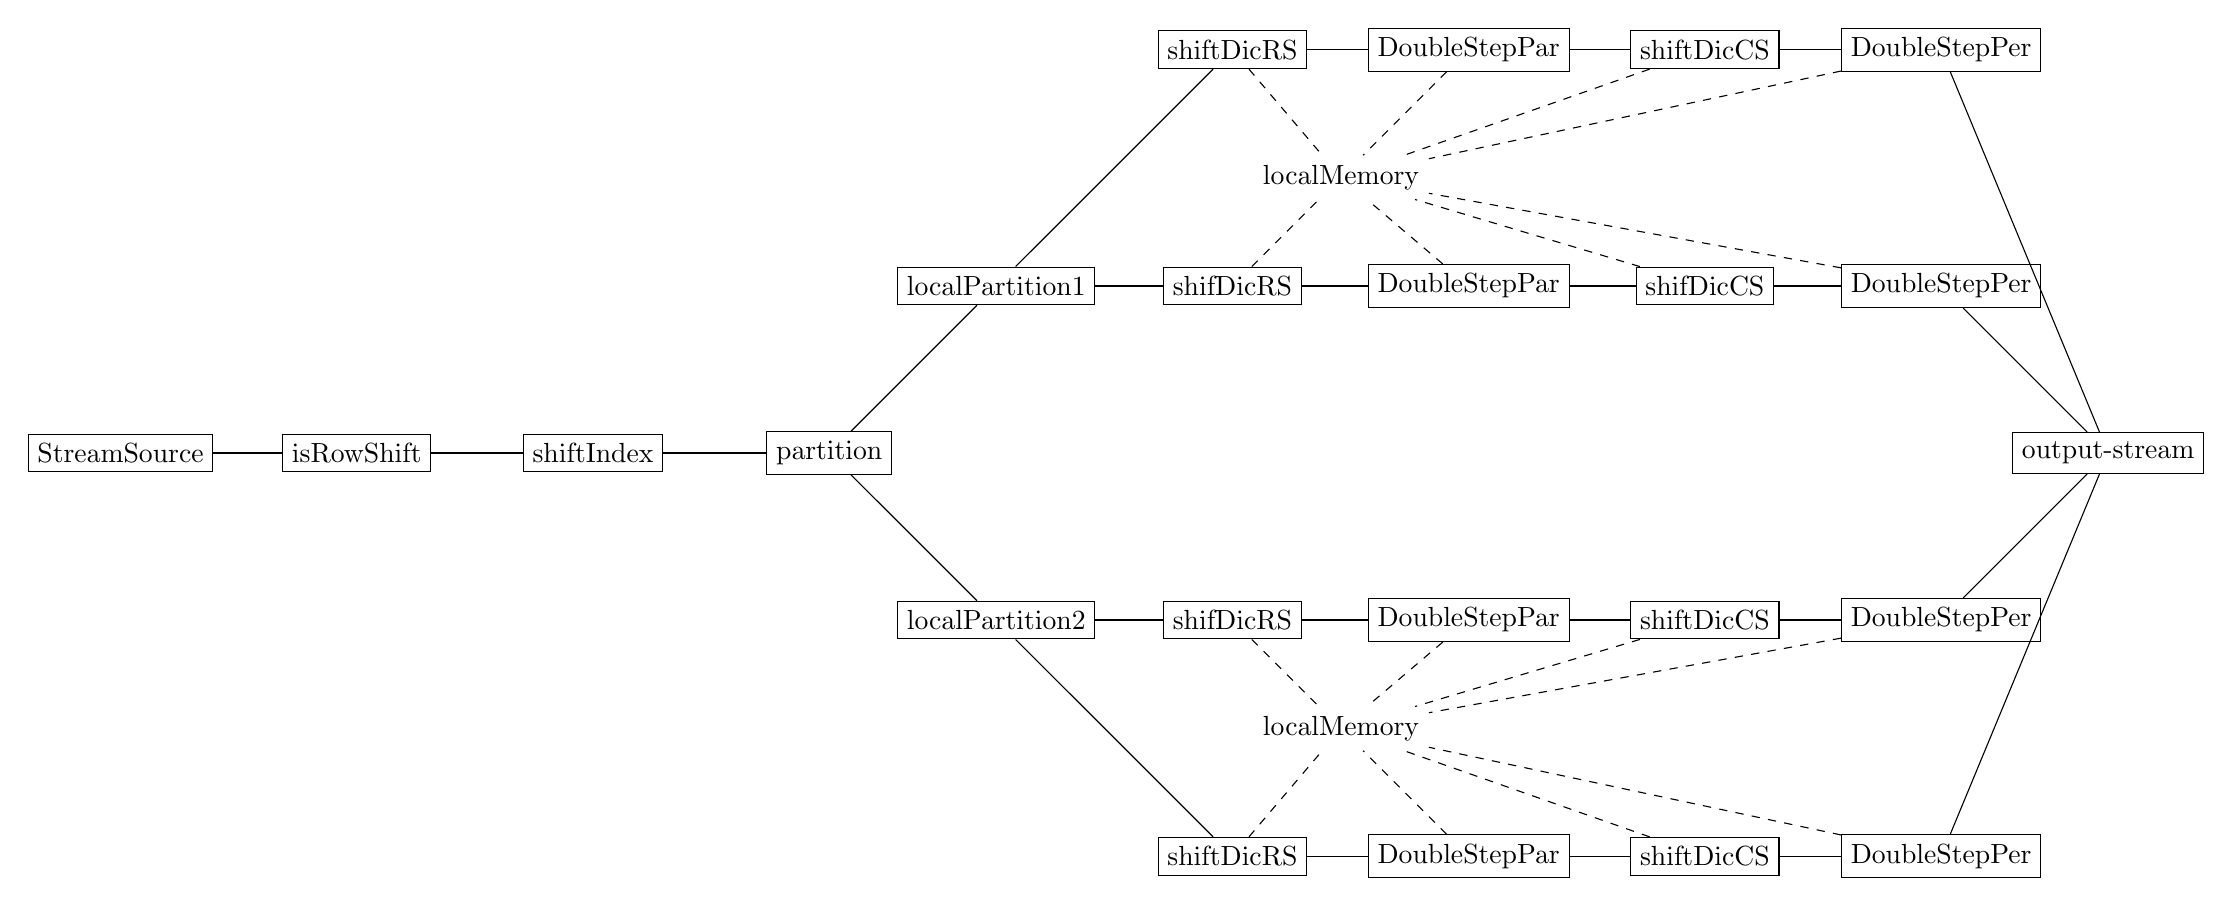
\begin{tikzpicture}[node distance={30mm}, main/.style = {draw, rectangle}, transform shape] 
\node[main] (1) {StreamSource};
\node[main] (2) [right of=1]{isRowShift};
\node[main] (3) [right of=2]{shiftIndex};
\node[main] (4) [right of=3]{partition};

\node[main] (lp1) [above right of=4]{localPartition1};
\node[main] (9) [right of=lp1]{shifDicRS};
\node[main] (10) [right of=9]{DoubleStepPar};
\node[main] (11) [right of=10]{shifDicCS};
\node[main] (12) [right of=11]{DoubleStepPer};

\node[main] (5) [above of=9]{shiftDicRS};
\node[main] (6) [right of=5]{DoubleStepPar};
\node[main] (7) [right of=6]{shiftDicCS};
\node[main] (8) [right of=7]{DoubleStepPer};

\node[main] (lp2) [below right of=4]{localPartition2};
\node[main] (13) [right of=lp2]{shifDicRS};
\node[main] (14) [right of=13]{DoubleStepPar};
\node[main] (15) [right of=14]{shiftDicCS};
\node[main] (16) [right of=15]{DoubleStepPer};

\node[main] (17) [below of=13]{shiftDicRS};
\node[main] (18) [right of=17]{DoubleStepPar};
\node[main] (19) [right of=18]{shiftDicCS};
\node[main] (20) [right of=19]{DoubleStepPer};

\node[main] (os) [below right of=12]{output-stream};

\node at(15.5,3.5) (sm1) {localMemory};
\node at(15.5,-3.5) (sm2) {localMemory};


\draw (1)--(2);
\draw (2)--(3);
\draw (3)--(4);
\draw (4)--(lp1);
\draw (lp1)--(5); \draw (5)-- (6);  \draw (6)-- (7); \draw (7)-- (8); \draw (8)--(os);
\draw (lp1)--(9); \draw (9)--(10);  \draw (10)-- (11); \draw (11)-- (12); \draw (12)--(os);

\draw (4)--(lp2);
\draw (lp2)--(13); \draw (13)--(14);  \draw (14)--(15); \draw (15)--(16); \draw (16)--(os);
\draw (lp2)--(17); \draw (17)--(18);  \draw (18)--(19); \draw (19)--(20); \draw(20)--(os);

\draw (5)--(sm1)[dashed]; \draw (6)--(sm1)[dashed]; \draw (7)--(sm1)[dashed]; \draw (8)--(sm1)[dashed];
\draw (9)--(sm1)[dashed]; \draw (10)--(sm1)[dashed]; \draw (11)--(sm1)[dashed]; \draw (12)--(sm1)[dashed];
\draw (13)--(sm2)[dashed]; \draw (14)--(sm2)[dashed]; \draw (15)--(sm2)[dashed]; \draw (16)--(sm2)[dashed];
\draw (17)--(sm2)[dashed]; \draw (18)--(sm2)[dashed];  \draw (19)--(sm2)[dashed];  \draw (20)--(sm2)[dashed];


\end{tikzpicture} 

}

\caption{Float-char SPIFT with shared memory and Doublestep}
\label{fig:floatDOUBLE}
\end{figure}

\section{ Doublestep }

The naive approach of calculating the final matrix is to add all the shifted values for every entry of the matrix. This leads to a lot of additions getting done multiple times. We developed the double-step algorithm to insure every addition only happens once.

\subsection{ Simple Doublestep }

Consider two shift-vectors $\vec{v}_1$ and $\vec{v}_2$ with shift-index $s_1$ and $s_2$ where $s_1 = s_2+\frac{N}{2}$ which are both row-shiftable. In the first row, $\vec{v}_1$ and $\vec{v}_2$ get added together $\vec{v}_1[0]+\vec{v}_2[0]$ ([*] denotes by how much the vector is shifted). On the next row, we get $\vec{v}_1[s_1]+\vec{v}_2[s_2]$. On the third row, it's $\vec{v}_1[2*s_1]+\vec{v}_2[2*s_2] = \vec{v}_1[2*s_1]+\vec{v}_2[2*s_1+2*\frac{N}{2}] = \vec{v}_1[2*s_1]+\vec{v}_2[2*s_1] = (\vec{v}_1[0]+\vec{v}_2[0])[2*s_1] $. And on the forth $\vec{v}_1[4*s_1]+\vec{v}_2[4*s_2] = (\vec{v}_1[s_1]+\vec{v}_2[s_1 +\frac{N}{2}])[2*s_1]$.\\

As we can see, we only need to make two vector-additions, $\vec{v}_1[0]+\vec{v}_2[0]$ and $\vec{v}_1[s_1]+\vec{v}_2[s_2]$. These two rows form a $2\times N$-matrix. If we shift this matrix by a multiple of $2*s_1$, it corresponds to the shifted addition of $v_1$ and $v_2$. We will call this matrix $sm_{2*s_1}^2$, where the subscript denotes the shift-index of the shift-matrix, and the superscript denotes the amount of rows it has. We can do this with all shift-vector-pairs to get $\frac{N}{2}$ shift-matrices, that all have an even shift-index.\\

Using all the $2\times N$-shift-matrices, we can use the same method to construct $\frac{N}{4}$ $4\times N$-matrices with shift-vectors that are multiple of four. We repeat this process until we have calculated $sm_{0}^N$, which is the final matrix.

\subsection{ Doublestep with parallelism }

As with the naive approach, using a parallel approach means slicing the image matrix into sub-matrices. Different then the naive approach though, all processes on the same machine handle one large slice, rather then one smaller slice per process on the machine. When setting up the pipeline, it still has to be decided if the image-matrix gets horizontally or vertically. Here I will assume it gets sliced horizontally, but the same system will also work with vertical slices.\\

Calculating the new image matrix slice when a new batch gets processed is split in two halves. First all shift-vectors with horizontal shift get added, then all shift-vectors with vertical shift. This order is arbitrary. Doublestep works differently, depending if the shift is parallel to the slicing or perpendicular to it. The different algorithms get discussed in the next two sections.

\subsubsection{ Parallel }

In this case, we consider row-shift and horizontal slicing. Let $D_i=\frac{N*lp_i}{gp}$ the size of the image-sub-grid that the machine i has to calculate and $l_{i,0}=\sum_{j=0}^{i-1}lp_i+1$ be the first line that this machine has to calculate (we start counting from 0). In this case we use Doublestep to calculate the first $\log{D_i}$ steps of Doublestep to get $\log{(N-D_i)}$ matrices of size $D_i \times N$.\\

We need all shift-vectors for this, so we have to calculate them beforehand. Since it is easier to calculate the shift-matrices if we assume we are handling the first row of the matrix, we will also shift all values $l_ {i,0}$ times, to emulate this. The calculation of the shift-vectors is evenly distributed among all local processes. Every process writes the result its shift-vectors to a block of memory of size  $\frac{N^2}{lp_i}$, that only it can write on, but others can read as well.\\

Algorithm \ref{fig:AlgoSVDoubleStepPara} shows how process $k\in \{0,1,2,...(lp_i-1)\}$ calculates the shift-vectors. \\

\begin{algorithm}
\caption{Calculating shift-vectors for parallel double-step}\label{euclid}
\label{fig:AlgoSVDoubleStepPara}
\begin{algorithmic}[1]
\State $r = N/lp_i$
\State $range = [k*r,(k+1)*r]$
\For{ vis in visibilities, vis.isRS and $vis.shiftIndex \in range$}
      \State q = emptyVector
      \For{ i $\leftarrow$ 0 to N  }
            \State $q[i]=vis.value*W^{(i*vis.v-l_{i,0}*vis.shiftIndex)\%N}$
      \EndFor
      \State memory.setShiftVector(vis.shiftIndex,q)
\EndFor
\end{algorithmic}
\end{algorithm}

The local processes now calculate the shift-matrices for each step together. We allocate a second blocks of memory of size $\frac{N^2}{lp_i}$ to each process. The first block is to store the result from the previous step (reading block), and the other block to calculate the next step (writing block). All processes have reading-rights to all memory blocks, but only writing rights to their own. Since every step only needs the shift-matrices of the previous one, after every step the previous reading block can become the new writing block.\\

Initially, there will be enough shift-matrices so that every process can calculate one or multiple full shift-matrices. Later, processes will calculate shift-matrices together, so the value of the shift-matrices will be distributed over multiple memory-blocks. Algorithm \ref{fig:AlgoDoubleStepParaSmall} shows how processes  $k\in \{0,1,2,...(lp_i-1)\}$ calculates the shift matrices in the j-th step of Doublestep ($1 \leq j\leq \log D_i,j\leq \log \frac{N}{lp_i})$ when it can calculate shift-matrices alone.\\

\begin{algorithm}
\caption{Partial parallel Doublestep Algorithm for process k for small j}\label{euclid}
\label{fig:AlgoDoubleStepParaSmall}
\begin{algorithmic}[1]
\State $r = N/(2^j*lp_i)$
\State $range = [k*r,(k+1)*r]$
\State $shiftIndexes = range*2^j$
\For{ shiftIndex in shiftIndexes }
      \State $m_1 = memory.getPreviousMatrix( \frac{shiftIndex}{2} )$
      \State $m_2 = memory.getPreviousMatrix( \frac{shiftIndex}{2}+\frac{N}{2} )$
      \State $firstHalf = m_1.shift(0) + m_2.shifted(0)$
      \State $secondHalf = m_1.shifted(\frac{shiftIndex}{2}) + m_2.shifted(\frac{shiftIndex}{2}+\frac{N}{2})$
      \State $memory.setNextMatrix( shiftIndex, concatenate(firstHalf,secondHalf)$
\EndFor
\end{algorithmic}
\end{algorithm}

When there are more processes then shift-matrices to calculate, multiple processes can start to calculate the same matrix. This can be done, because the calculation of every row in a shift-matrix is independent from all other rows. Processes still store the partial-shift-matrix in there own memory-block, to avoid problems with parallel access.  Algorithm \ref{fig:AlgoDoubleStepParaBig} shows how processes  $k\in \{0,1,2,...(lp_i-1)\}$ calculates the shift matrices in the j-th step of Doublestep ($1 \leq j\leq \log D_i,j> \log \frac{N}{lp_i})$ when it needs to cooperate with other processes.\\

\begin{algorithm}
\caption{Partial parallel Doublestep Algorithm for process k for big j}\label{euclid}
\label{fig:AlgoDoubleStepParaBig}
\begin{algorithmic}[1]
\State $r = \frac{N}{2^j*lp_i}$
\State $number = int(k*r)$
\State $lines = [(k*r-number)*2^j,((k+1)*r-number)*2^j]$
\State $shiftIndex =number*2^j$
\For{ line in lines }
      \If {$line < \frac{2^j}{2}$}
          \State $l_1 = memory.getLineOfPreviousMatrix( \frac{shiftIndex}{2}, line )$
          \State $l_2 = memory.getLineOfPreviousMatrix( \frac{shiftIndex}{2}+\frac{N}{2},line )$
          \State $memory.setLineOfNextMatrix(shiftIndex, line, l_1+l_2)$
      \Else
          \State $l_1 = memory.getLineOfPreviousMatrix( \frac{shiftIndex}{2}, ((line-\frac{N}{2})-(\frac{shiftIndex}{2}))\%N )$
          \State $l_2 = memory.getLineOfPreviousMatrix( \frac{shiftIndex}{2}+\frac{N}{2},((line-\frac{N}{2})-(\frac{shiftIndex}{2}+\frac{N}{2}))\%N)$
          \State $memory.setLineOfNextMatrix(shiftIndex, line, l_1+l_2)$      
      \EndIf
\EndFor
\end{algorithmic}
\end{algorithm}

In the end, all shift-matrices of size $D_i \times N$ need to be added to the previous image-sub-Grid to. Every process can handle it's own sub-Grid, and asses the $D_i \times N$ matrices, since every process has read-access. Let $NrLines$ be the number of lines each process has to handle. Algorithm \ref{fig:AlgoDoubleStepFinal} shows how process k calculates its sub-grid.

\begin{algorithm}
\caption{Partial parallel Doublestep Algorithm for process k, calculating final}\label{euclid}
\label{fig:AlgoDoubleStepFinal}
\begin{algorithmic}[1]
\State $lines = [0 ,NrLines]$
\For{ line in lines }
      \State $rowToAdd = memory.getLineOfPreviousMatrix(0, k*NrLines+line)$
      \For{$ i \leftarrow 1$ to $\frac{N}{D_i} $ }
             \State $rowToAdd \mathrel{+}= memory.getLineOfPreviousMatrix(i*2^j, k*NrLines+line)$
      \EndFor
      \State $memory.setLineOfSubGrid(line, rowToAdd + memory.getLineOfSubGrid(line) )$
\EndFor
\end{algorithmic}
\end{algorithm}

\subsubsection{ Perpendicular }
In this case we consider column-shift and horizontal slicing.  Let $D_i=\frac{N*lp_i}{gp}$ the size of the image-sub-grid that the machine i has to calculate and $l_{i,0}=\sum_{j=0}^{i-1}lp_i+1$ be the first line that this machine has to calculate (we start counting from 0).\\


Like in the parallel-case, the processes will now calculate the shift-dictionary and the steps of Doublestep together. What differs from the parallel case, is that all steps of Doublestep will get calculated, and that not all lines will be considered, since not all lines matter for the final image-sub-grid (Figure \ref{fig:doubleStep}). Before we start calculating the steps of Doublestep, we calculate what lines are needed in each shift-matrix. To do this, we first consider the final $D_i \times N$-Matrix. It will need all the lines in the range $[l_{i,0},l_{i,0}+D_i]$. To calculate it, we need the lines $[l_{i,0},l_{i,0}+D_i]$ of the shift-matrix with shift-index 0 and size $N \times \frac{D_i}{2}$, and the lines $[l_{i,0},l_{i,0}+D_i] \cup [l_{i,0}+\frac{N}{2},l_{i,0}+D_i+\frac{N}{2}]$. In general, to calculate the lines of set $l$ for a shift matrix of size $N \times B$ with shift-index s, we need the following lines from the shift-matrices of size $N \times \frac{B}{2}$: From the matrix with shift index $\frac{s}{2}$ we need the lines of set $l \cup l+\frac{s}{2}$ and from the shift-matrix with shift-index $\frac{s+N}{2}$ we need lines of set $l \cup l+\frac{s+N}{2}$. Using this formula we can recursively calculate all lines we need for each shift-matrix, as seen in Algorithm \ref{fig:RecusriveLines}.\\

\begin{figure}[ht]
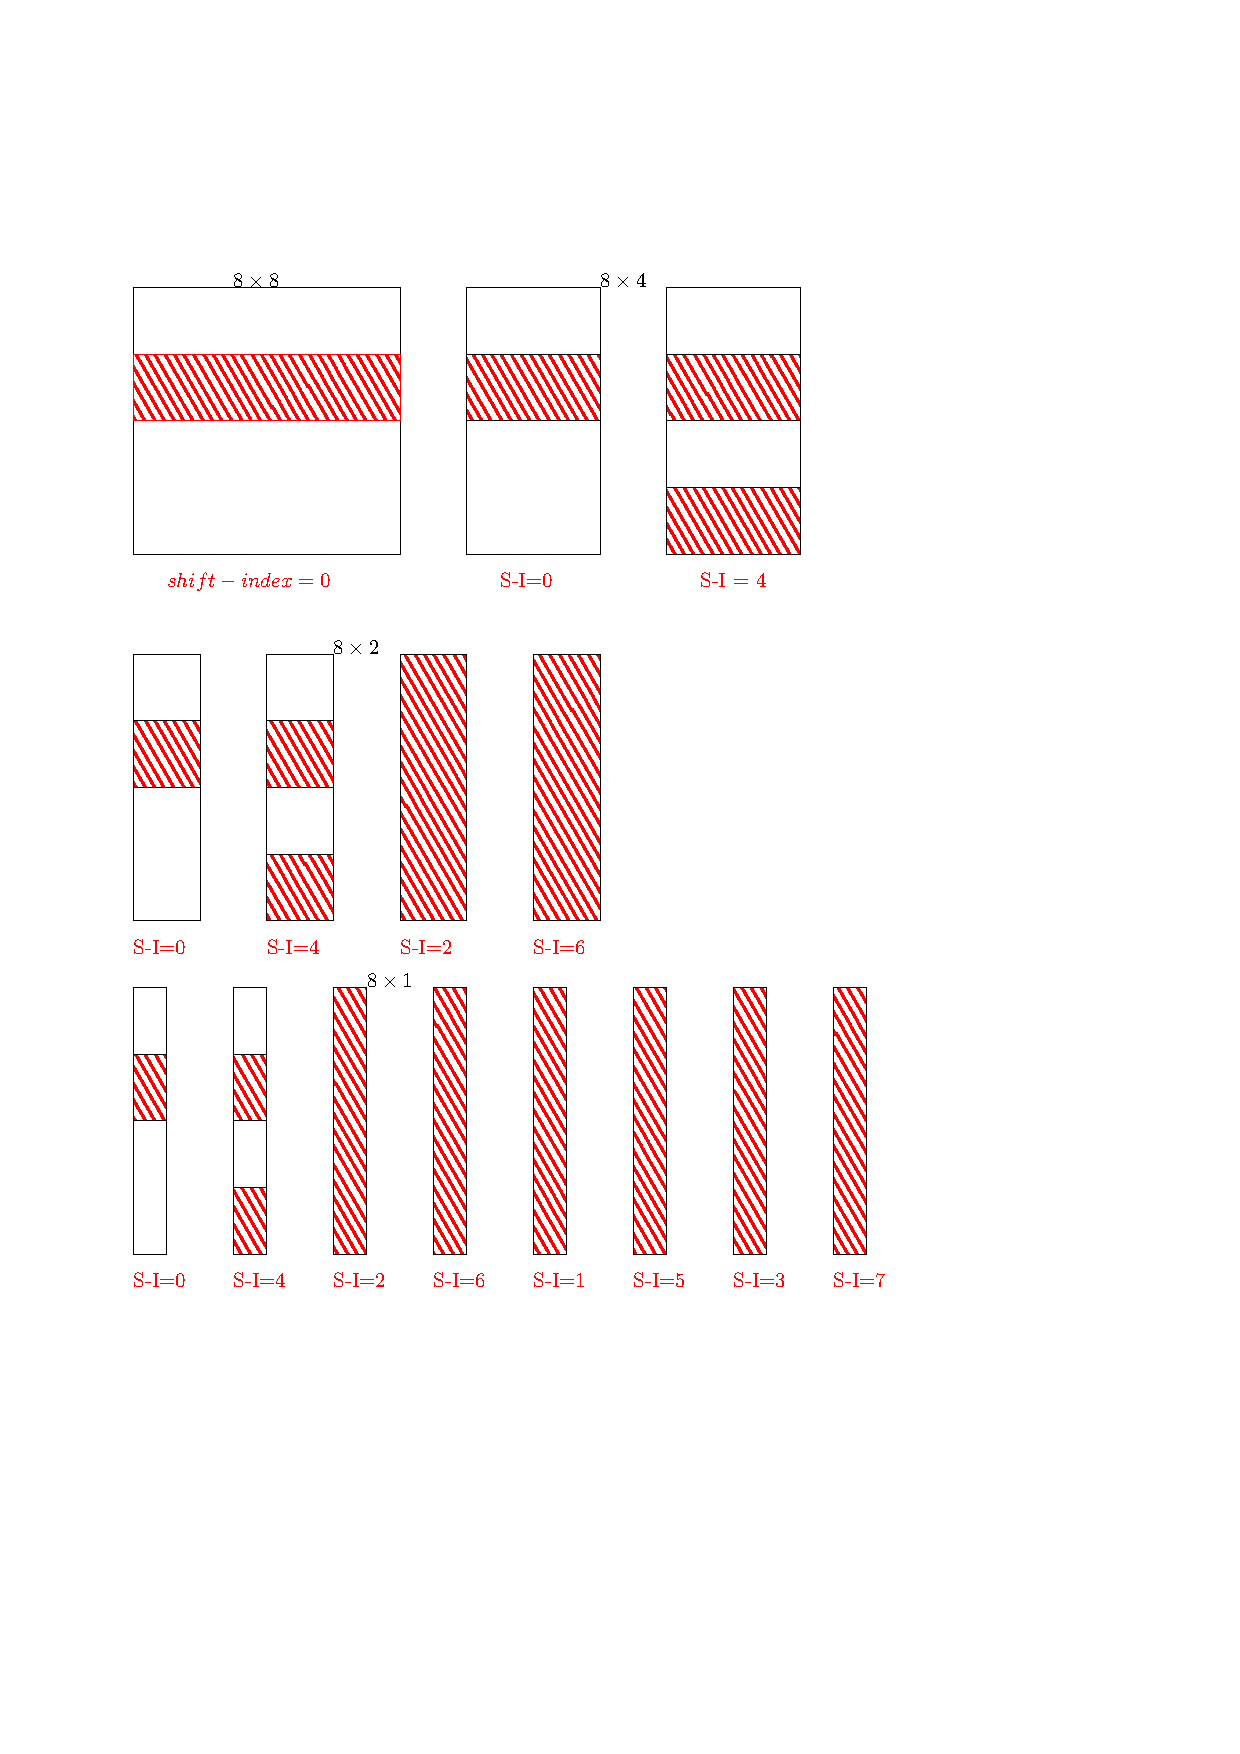
\includegraphics{doubleStepPerpendicular}
\caption{Cool caption}
\label{fig:doubleStep}
\end{figure}


\begin{algorithm}
\caption{Calculating needed lines for shift-matrices}\label{euclid}
\label{fig:RecusriveLines}
\begin{algorithmic}[1]
\State $MatrixSizeDic = dic()$
\State $D = N$
\State $originalLines = \{l_{i,0},l_{i,0}+1,...,l_{i,0}+D_i-1\}$
\State $originalShiftMatrixDic = dic( 0: originalLines )$
\State $MatrixSizeDic[N] = originalShiftMatrixDic$
\State $D = \frac{D}{2}$
\While{ $D \leq 1$}
        \State $newLinesDic = dic()$
        \For {shiftIndex in MatrixSiteDic[2*D].keys}
             \State $lines = MatrixSiteDic[2*D][shiftIndex]$
             \State $newLinesDic[\frac{shiftIndex}{2}] = lines \cup lines+\frac{shiftIndex}{2}$
             \State $newLinesDic[\frac{shiftIndex+N}{2}]= lines \cup lines+\frac{shiftIndex+N}{2}$
        \EndFor
        \State $MatrixSizeDic[D] = newLinesDic$
        \State $D = \frac{D}{2}$
\EndWhile
\end{algorithmic}
\end{algorithm}

Now that we know what lines are needed, we can start to calculate them. Since the amount of lines one shift-vector needs can vary by a lot, we can't just allocate the vectors to different processes and assume they will all have to do the same amount  of work. Instead, we will create a list of all values that need to be calculated in all vectors, and then divide that list evenly between processes. Then each process will calculate one equal chunk of that list (Algorithm \ref{fig:PerpenSVDS}).\\

\begin{algorithm}
\caption{Calculating shift-vectors for parallel double-step by process k}\label{euclid}
\label{fig:PerpenSVDS}
\begin{algorithmic}[1]
\State $list = []$
\For {shiftIndex in MatrixSizeDic[1].keys}
     \For {line in MatroxSizeDic[1][shiftIndex]}
          list.add( (shiftIndex,line) )
     \EndFor
\EndFor

\State $chunkSize = roundedUp( \frac{list.size}{lp_i} )$
\For {$ i \leftarrow k*chunkSize$ to $(k+1)*chunkSize$}
     \State shiftIndex, line = list[i]
     \State vis = visibilities.get(shiftIndex)
     \State $memory.set( shiftIndex, line, vis.value*W^{line*vis.u} )$
\EndFor
\end{algorithmic}
\end{algorithm}

Now that the shift-vectors are calculated, we can proceed to calculate the shift-matrices. The process is basically the same. Make a list of all rows that need to be calculated, divide the list evenly among th processes and then calculate them (Algorithm \ref{fig:PerpenDS}).


\begin{algorithm}
\caption{Calculating the j-th step for perpendicular double-step by process k}\label{euclid}
\label{fig:PerpenDS}
\begin{algorithmic}[1]
\State $list = []$
\For {$shiftIndex in MatrixSizeDic[2^j].keys$}
     \For {$line in MatroxSizeDic[2^j][shiftIndex]$}
          list.add( (shiftIndex,line) )
     \EndFor
\EndFor

\State $chunkSize = roundedUp( \frac{list.size}{lp_i} )$
\For {$ i \leftarrow k*chunkSize$ to $(k+1)*chunkSize$}
     \State shiftIndex, line = list[i]
      \If {$line < \frac{2^j}{2}$}
          \State $l_1 = memory.getLineOfPreviousMatrix( \frac{shiftIndex}{2}, line )$
          \State $l_2 = memory.getLineOfPreviousMatrix( \frac{shiftIndex}{2}+\frac{N}{2},line )$
          \State $memory.setLineOfNextMatrix(shiftIndex, line, l_1+l_2)$
      \Else
          \State $l_1 = memory.getLineOfPreviousMatrix( \frac{shiftIndex}{2}, ((line-\frac{N}{2})-(\frac{shiftIndex}{2}))\%N )$
          \State $l_2 = memory.getLineOfPreviousMatrix( \frac{shiftIndex}{2}+\frac{N}{2},((line-\frac{N}{2})-(\frac{shiftIndex}{2}+\frac{N}{2}))\%N)$
          \State $memory.setLineOfNextMatrix(shiftIndex, line, l_1+l_2)$      
      \EndIf
\EndFor
\end{algorithmic}
\end{algorithm}


In the end, all image-sub-Grid need to be updated. Every process can handle it's own sub-Grid, and access the final shift-matrix, since every process has read-access. Let $NrLines$ be the number of lines each process has to handle (Algorithm \ref{fig:PerpenDSfinal}). 

\begin{algorithm}
\caption{Partial perpendicular Doublestep Algorithm for process k, calculating final}\label{euclid}
\label{fig:PerpenDSfinal}
\begin{algorithmic}[1]
\State $lines = [0 ,NrLines]$
\For{ line in lines }
      \State $rowToAdd = memory.getLineOfPreviousMatrix(0, k*NrLines+line)$
      \State $memory.setLineOfSubGrid(line, rowToAdd + memory.getLineOfSubGrid(line) )$
\EndFor
\end{algorithmic}
\end{algorithm}

\section{ Calculation }

Doublestep with parallel processes and shared memory takes $\log{\frac{N}{gp}}*\frac{N^2}{max(\{lp_0,...,lp_{gp-1}\})}$ complex additions and less then $\frac{3}{2}N^2$ complex additions.

\end{document}
